\section{Conclusion}
\label{section:conclusion}

We presented a training-free, inversion-free image editing framework that brings
attention-driven spatial control to Visual Autoregressive Models. Cross-attention
maps inside a VAR transformer already carry enough spatial semantics to build
precise editing masks, provided that blocks dominated by positional bias are
removed and that the maps are binarized by an absolute energy level rather than
by rank; combined with the self-consistency of BSQ tokenization, this yields
background preservation by construction instead of by approximation.

Beyond the method itself, our analysis isolates what actually governs the
preservation--edit trade-off in this setting. The base threshold level traces a
smooth, monotone frontier and is the single control worth exposing; the
CV-adaptive correction shifts that frontier outward by an amount we quantify
against the fixed-threshold interpolation under two independent preservation
metrics; the target-stream pass contributes structurally rather than
parametrically, moving the entire frontier rather than the operating point along
it; explicit coarse anchoring dominates the implicit cumulative alternative; and
the preserve level, despite appearing as a hyperparameter, provably cannot affect
the output.

We believe the discrete, scale-wise structure of autoregressive generation is a
promising and still underexplored foundation for training-free image
manipulation, and that the mask construction demonstrated here transfers directly
to autoregressive video generation, where the same coarse-to-fine schedule
applies frame by frame.

\begin{figure}[t]
    \centering
    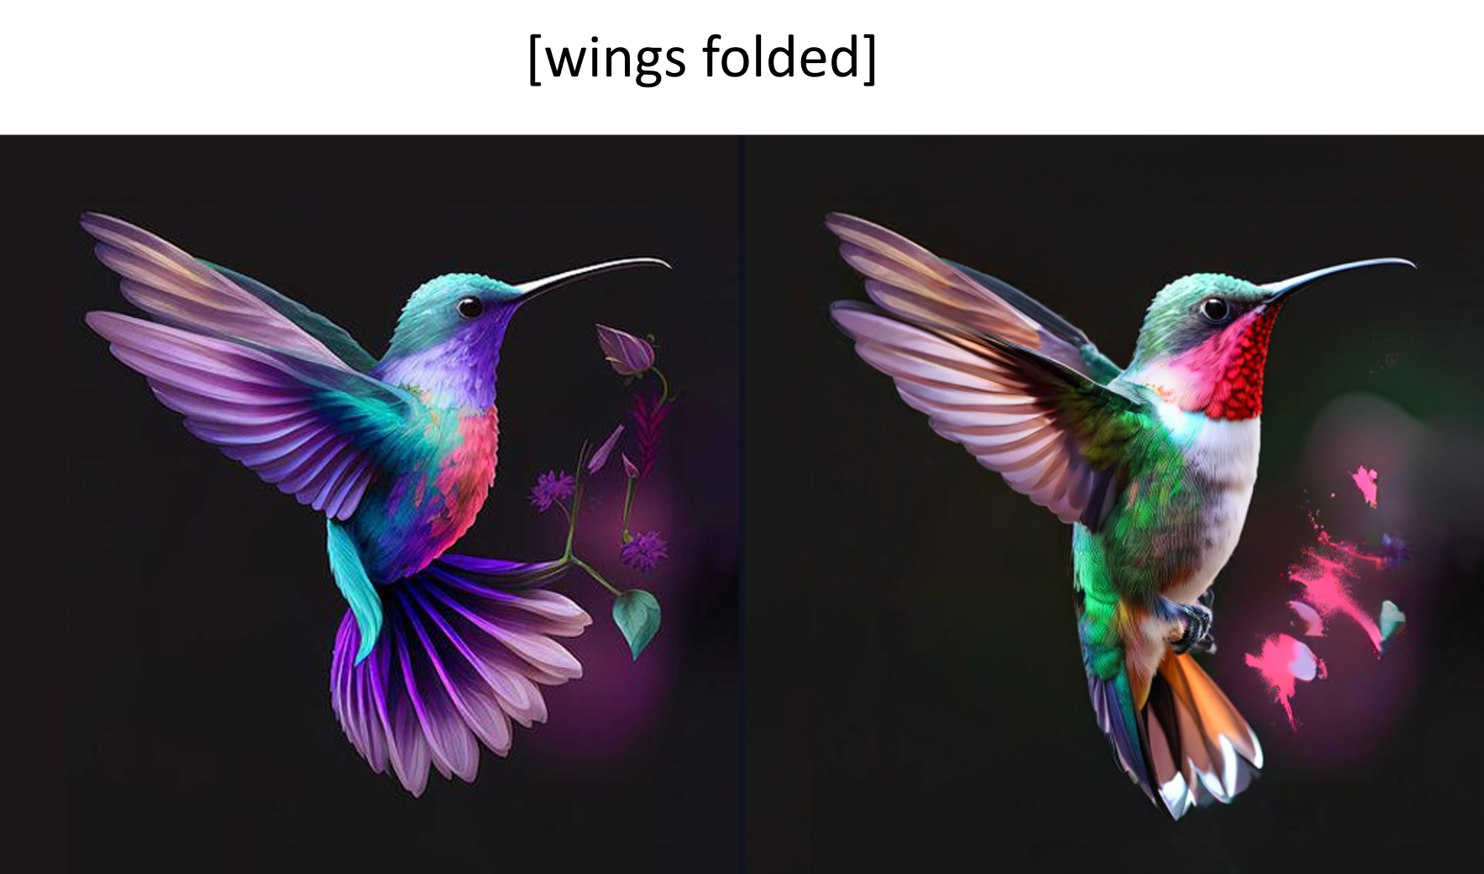
\includegraphics[width=0.75\linewidth]{imgs/failure_cases.png}
    \caption{Failure case: drastic pose changes conflict with coarse-scale structural anchoring.}
    \label{fig:failure_cases}
\end{figure}
